%---------------------------------------------------------------------------------------------------------------%
\section{Fase --- C}
%---------------------------------------------------------------------------------------------------------------%
Nesta fase, implementou-se o grupo da tabela de números hexadecimais.  Como já
foi anteriormente dito, o código foi gerado a partir da MIB, com
o \emph{AgentPro}, e dividido em mais classes. A partir do código gerado pôde-se
construir as classes \texttt{UnpredictableTableEntryRow}, que serviu para criar
uma linha na tabela de números hexadecimais (índice e numero hexadecimal), 
e a classe \texttt{UnpredictableTableEntryRowFactory} que aplica a classe
anterior com o método \texttt{createRow}. Note-se que, este método recebe o OID
da linha, bem como um \emph{array} de \texttt{Variable}, naturalmente de tamanho
2 (índice e valor).

À semelhança do que se fez na fase anterior, obtiveram-se partes do código
gerado, para construir uma nova classe, de nome \texttt{MOTableBuilder}. Esta
classe instancia objetos necessários à constituição da tabela, como sub-índices,
índices e utiliza um modelo para a construção da tabela. Nesta classe, há
a salientar dois métodos: \texttt{addValue} e \texttt{build}. O método
\texttt{addValue} adiciona valores a um \emph{array} de \emph{arrays} de
\texttt{Variable}, numa variável da classe. De cada vez que um número
hexadecimal é adicionado, é adicionado num \emph{array} de \texttt{Variable} de
duas colunas, onde o índice é controlado por uma variável de classe de valor
inteiro, sendo o índice e o valor hexadecimal adicionados ao \emph{array}.
Quando o método \texttt{build} é invocado, esta variável é reinicializada.

O método \texttt{build} cria a definição de sub-índice onde o OID do índice da
tabela e o índice com base nos sub-índices definidos.  Na criação das colunas,
a coluna do índice da tabela tem as permissões de acesso alteradas para
\emph{ACESSIBLE\_FOR\_READ\_ONLY}. Na coluna do número hexadecimal, é atribuído,
o tipo \texttt{DisplayString} com permissões de
\emph{ACESSIBLE\_FOR\_READ\_WRITE}.  A tabela é criada, sem valores, onde depois
é adicionado à tabela todos os valores guardados, através do método
\texttt{addValue}.  À luz do que se fez na fase B, também se implementou um
interface \texttt{MOGroup} pelos mesmos motivos já descritos.

Na classe \texttt{AgentHelper}, cujo intuito é partilhar entre instâncias de classes
e processos, a informações de estado e configuração, adicionou-se um método para
carregamento do ficheiro das \emph{sementes} iniciais.

No método \texttt{main}, antes da criação do grupo dos objetos escalares,
implementou-se o método de carregamento das sementes sendo a classe
\texttt{MOTableBuilder} instanciada, os valores das \emph{sementes} adicionados
à instancia daquela classe, sendo a tabela construída e registada, como o grupo
de objetos escalares na fase B.


\subsection{Testes}

\begin{center}
 	
 	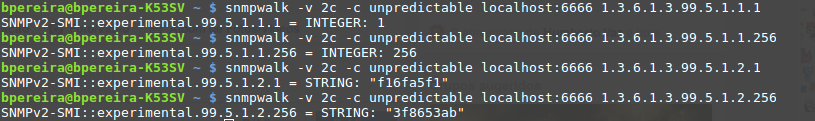
\includegraphics[width=\textwidth,height=\textheight,keepaspectratio]{resources/images/faseC/faseC.png}
 	\captionsetup{type=figure, width=0.8\linewidth}
	\caption{Testes}
\label{fig:faseB:teste} 
\end{center}



